\documentclass{beamer}
\usetheme{Boadilla}

\usepackage{graphicx}
\graphicspath{{./images/}}

\title{Relatório do EP2}
\subtitle{MAC0422 - Sistemas Operacionais (2024)}
\author{Gabriel Takeuchi - NUSP: 13671636}
\date{}

\begin{document}

% Capa
\begin{frame}
  \titlepage
\end{frame}

\section{Implementação}

\subsection{Ciclistas}
\begin{frame}
  \frametitle{Os ciclistas}
  \begin{itemize}
    \item Há um array dinâmico global de ciclistas \texttt{ciclistas} com tamanho $k$.
    \item Cada ciclista é uma \texttt{struct} \texttt{Ciclista} com os campos:
    \begin{itemize}
      \item \texttt{int id}: identificador único (de 0 a $k$)
      \item \texttt{int posicao\_x, posicao\_y}: metro e raia atual
      \item \texttt{int velocidade}: velocidade atual
      \item \texttt{int voltas}: quantas voltas deu em relação a ele
      \item \texttt{int colocacao}: colocação final (alterada apenas quando ganha ou quebra)
      \item \texttt{double tempo\_final}: em quanto tempo em segundos ganhou a corrida (não é calculado se ele quebrou)
      \item \texttt{bool na\_corrida}
      \item \texttt{bool atualizou\_posicao}: usado para coordenar se o ciclista deve andar em um ciclo
    \end{itemize}
  \item Para acessar os ciclistas, utilizamos um mutex \texttt{mutex\_ciclistas}.
  \end{itemize}
\end{frame}

\subsection{As threads}
\begin{frame}{As threads}
  \begin{itemize}
    \item Há um array dinâmico global de threads \texttt{threads} com tamanho $k$.
    \item Cada thread corresponde exatamente a um ciclista.
    \item As threads são criadas e executam a função \texttt{f\_ciclista(void *arg)}, sendo \texttt{arg} o inteiro identificador do ciclista que corresponde à thread.
    \item Para que as barreiras de sincronização funcionem, as threads encerram com \texttt{pthread\_exit(NULL)} apenas quando a corrida acaba.
  \end{itemize}
\end{frame}

\subsection{A pista}
\begin{frame}
  \frametitle{A pista}
  \begin{itemize}
    \item A \texttt{pista} é uma matriz de dimensões $d \times 10$, sendo $d$ o tamanho da pista em metros. Acessamos o elemento no metro $x$ e raia $y$ com \texttt{pista[x][y]}.
    \item Mentalize a pista como o primeiro quadrante de um plano cartesiano, onde a origem é o canto inferior esquerdo.
    \item Para acessar a \texttt{pista}, utilizamos um mutex \texttt{mutex\_pista}.
  \end{itemize}
\end{frame}

\subsection{A largada}
\begin{frame}
  \frametitle{A largada}
  \begin{itemize}
    \item Seja $k$ o número de ciclistas.
    \item A largada é organizada com grupos de 5 ciclistas lado-a-lado em cada metro
    \item Os ciclistas de cada grupo são inicializados nas raias 0 à 4.
    \item O primeiro grupo é inicializado no metro 0, o segundo no metro 1, $\dots$, até o metro $\lceil\frac{k}{5}\rceil$.
    \item Resumo: temos $\lceil\frac{k}{5}\rceil$ colunas de 5 ciclistas.
  \end{itemize}
\end{frame}

\subsection{Loop principal}
\begin{frame}
  \frametitle{Loop principal}
  \begin{itemize}
    \item Utilizamos 2 barreiras de sincronização:
    \begin{itemize}
      \item A \texttt{barreira\_ciclistas\_andaram} sincroniza as threads para executarem.
      \item A \texttt{barreira\_impressao} impede que as threads executem enquanto a \texttt{main} imprime e processa os dados.
    \end{itemize}
    \item O loop principal segue a seguinte lógica:
    \begin{enumerate}
      \item As threads executam e os ciclistas fazem suas operações.
      \item As threads sincronizam na \texttt{barreira\_ciclistas\_andaram}, e esperam na \texttt{barreira\_impressao}.
      \item O loop principal verifica quem ganhou e quebrou e imprime a situação atual da corrida.
      \item O loop principal sincroniza na \texttt{barreira\_impressao} e, caso exista ciclista na pista, libera as threads para a próxima iteração.
    \end{enumerate}
  \end{itemize}
\end{frame}

\subsection{Fim da corrida}
\begin{frame}{Fim da corrida}
  \begin{itemize}
    \item A corrida finaliza apenas quando o último ciclista ganha ou quebra.
    \item O tempo final de cada ciclista é calculado em segundos.
  \end{itemize}
\end{frame}

\subsection{Saídas}
\begin{frame}
  \frametitle{Saídas}
  \begin{itemize}
    \item Modo debug:
    \begin{itemize}
      \item A pista \textbf{inteira} é impressa no terminal a cada tick. Não é recomendado para pistas grandes.
      \item Para limpar a tela a cada tick, descomente a linha 414 do arquivo \texttt{ep2.c} na função \texttt{imprime\_corrida\_debug()}. Caso contrário, todas as impressões serão normalmente feitas a cada tick.
      \begin{itemize}
        \item A linha comentada é \texttt{printf(\textbackslash033[H\textbackslash033[J);}
      \end{itemize}
      \item O resultado final é escrito no arquivo \texttt{saida.txt}
    \end{itemize}
    \item Modo normal:
    \begin{itemize}
      \item Nada é impresso no terminal.
      \item Todos os resultados de cada volta e final são escritos no arquivo \texttt{saida.txt}
    \end{itemize}
  \end{itemize}
\end{frame}

\section{Testes}

\subsection{Gráficos}
\begin{frame}
  \frametitle{Gráficos de consumo de tempo}
  \begin{figure}
    \centering
    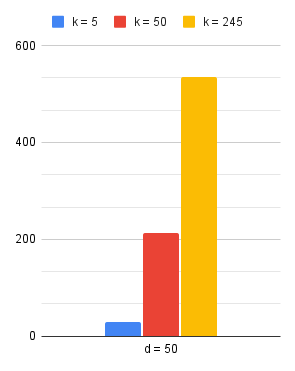
\includegraphics[width=0.3\textwidth]{t_d_peq.png}
    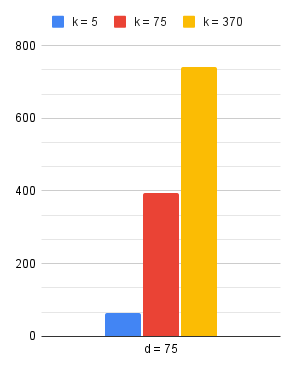
\includegraphics[width=0.3\textwidth]{t_d_med.png}
    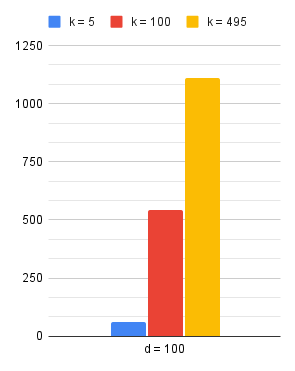
\includegraphics[width=0.3\textwidth]{t_d_gra.png}
  \end{figure}
  Obs.: As medições foram feitas em segundos.
\end{frame}

% \begin{frame}
%   \frametitle{Gráficos de consumo de RAM}
%   \begin{figure}
%     \centering
%     \includegraphics[width=0.33\textwidth]{r_d__peq.png}
%     \includegraphics[width=0.33\textwidth]{r_d__med.png}
%     \includegraphics[width=0.33\textwidth]{r_d__gra.png}
%   \end{figure}
% \end{frame}

\subsection{Análise}
\begin{frame}
  \frametitle{Análise do consumo de tempo}
  \begin{itemize}
    \item Consideramos $d = 50$ pequeno, $d = 75$ médio e $d = 100$ grande. Isto pois os tempo de execução ficariam absurdamente inviáveis de calcular para o intervalo $100 <= d <= 2500$.
    \item Os gráficos para todos os $d$ seguem uma tendência exponencial.
  \end{itemize}
\end{frame}

\end{document}
